\documentclass[12pt, twoside]{article}
% \documentclass[12pt, twoside]{article}
\usepackage[letterpaper, margin=1in, headsep=0.2in]{geometry}
\setlength{\headheight}{0.6in}
%\usepackage[english]{babel}
\usepackage[utf8]{inputenc}
\usepackage{microtype}
\usepackage{amsmath}
\usepackage{amssymb}
%\usepackage{amsfonts}
\usepackage[nomessages]{fp} %\FPeval{\var-name}{2*sin(pi/6)}
\usepackage{siunitx} %units in math. eg 20\milli\meter
\usepackage{yhmath} % for arcs, overparenth command
\usepackage{tikz} %graphics
\usetikzlibrary{quotes, angles, arrows, arrows.meta}
\usepackage{graphicx} %consider setting \graphicspath{{images/}}
\usepackage{parskip} %no paragraph indent
\usepackage{enumitem}
\usepackage{multicol}
\usepackage{venndiagram}

\usepackage{fancyhdr}
\pagestyle{fancy}
\fancyhf{}
\renewcommand{\headrulewidth}{0pt} % disable the underline of the header
\raggedbottom
\hfuzz=2mm %suppresses overfull box warnings

\usepackage{hyperref}
\usepackage{float}

\title{Algebra 2}
\author{Chris Huson}
\date{January 2025}

\fancyhead[LE]{\thepage}
\fancyhead[RO]{\thepage \\ First \& last name: \hspace{2.25cm} \,\\ Section: \hspace{2.25cm} \,}
\fancyhead[LO]{BECA / Huson / Precalculus: Transformations \\* 17 March 2025}

\begin{document}

\begin{enumerate}
    \setcounter{enumi}{7}

\item Simplify to the form $a+bi$ with $a,b$ real numbers. \hfill \emph{N.CN.2 Complex numbers}
    \begin{multicols}{2}
        \begin{enumerate}[itemsep=1.5cm]
            \item $(6 + 2i) - (7 - 5i)$
            \item $(x - 2i)(2 + 3i)=$
        \end{enumerate}
    \end{multicols}  \vspace{3cm}

\item Simplify each expression, using imaginary numbers as necessary.
    \begin{multicols}{2}
    \begin{enumerate}[itemsep=0.5cm]
        \item $\sqrt{-9}=$
        \item $\displaystyle \frac{1}{2} \sqrt{-24}=$
    \end{enumerate}
    \end{multicols} \vspace{1cm}


\item Write down the solutions to \hfill \emph{F.IF.7c Graph polynomials, identify zeros} \\
$x(x -7)(2x + 5) = 0$
\vspace{2cm}

\item Write down the polynomial function shown in the graph in factored form. 
\begin{flushright}
    \begin{tikzpicture}[scale=0.5]
        \draw[lightgray,very thin] (-5,-10) grid (7,8);
        \draw [thick,<->] (-5.5,0)--(7.5,0) node [right] {$x$};
        \draw [thick,<->] (0,-10.5)--(0,8.5) node [below right] {$f(x)$};
        \foreach \x in {-4,-2, 2, 4,6}
            \draw[thick] (\x cm,5pt) -- (\x cm,-5pt) node[below] {$\x$};
        \foreach \y in {-2}
            \draw[thick] (4pt,\y cm)--(-4pt,\y cm) node[left]{$-10$};
        \draw [thick, <->, smooth,domain=-2.4:5.3] plot(\x,{0.2*(\x-1)*(\x-1)*(\x+2)*(\x-5)});
    \end{tikzpicture}
    \end{flushright}

       
\end{enumerate}
\end{document}